\documentclass{beamer}
\usepackage[utf8]{inputenc}
\usepackage[T1]{fontenc}
\usepackage{hyperref}
\usepackage{graphicx}
\title{Update on the Dynamic Federation}
\date[ISPN ’80]{Technical Coordination Board}
\author[Euclid]{Frank Berghaus \href{mailto:berghaus@cern.ch}{\texttt{berghaus@cern.ch}}}

% --- Blocks ---
\setbeamertemplate{blocks}[default]

\usetheme{frank}

\begin{document}

\begin{frame}
\titlepage
\end{frame}


\begin{frame}
\frametitle{Review: What does DynaFed do?}
\begin{itemize}
\item Aggregates storage and metadata farms on-the-fly
\item Exposes standard protocols that support redirections and WAN data access
\item Creates (the illusion of) a unique namespace from a set of distinct storage or metadata endpoints
\item read and write support
\end{itemize}
\end{frame}

\begin{frame}
  \frametitle{Dynafed Namespace}
  \begin{figure}
      \centering
      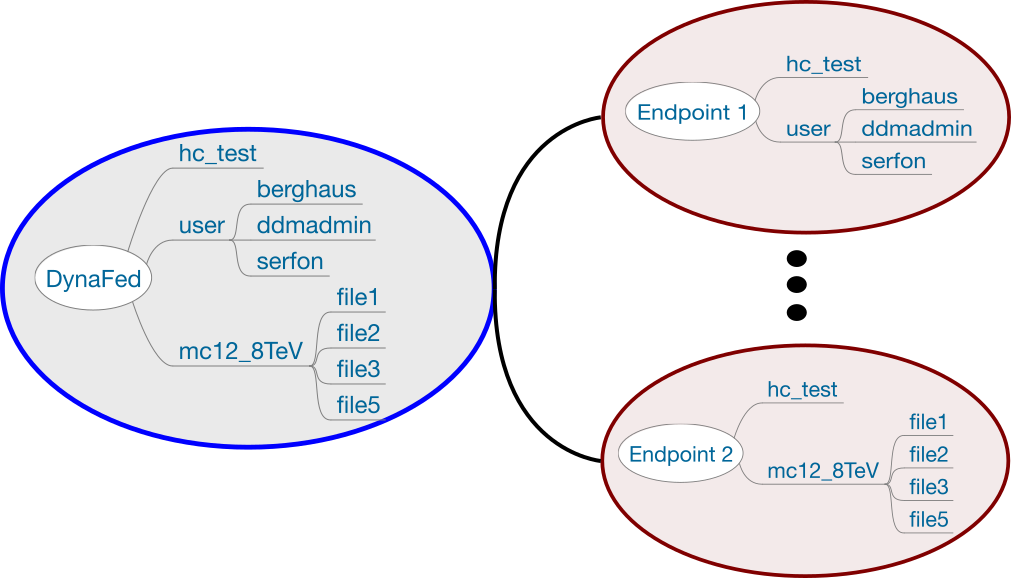
\includegraphics[width=\columnwidth]{dynafed-namespaces.png}
  \end{figure}
\end{frame}

\begin{frame}
  \frametitle{Motivation}
  \begin{itemize}
    \item Ease of negotiating connections between storage and users/jobs
    \item Integrate multiple storage backend under the same protocol
    \item Stability because of multiplication of data sources
    \item Ease the pain of supporting SRM
    \item What have I forgotten?
  \end{itemize}
\end{frame}

\begin{frame}
  \frametitle{ATLAS Projects with DynaFed}
  \begin{itemize}
    \item UVic in Victoria: Rolf Seuster \& Marcus Ebert
    \item UVic at CERN: Frank Berghaus
    \item At RAL: Alastair Dewhurst
    \item Italy in Frascati, Napoli and Roma: Alessandro De Salvo
  \end{itemize}
  With lots of help from ADC (Ale and Ivan) and DDM (Mario and Cedric)!
\end{frame}

\begin{frame}
  \frametitle{Status of DynaFed at CERN}
  \begin{itemize}
    \item Endpoint: \url{https://dynafed-dev.cern.ch/atlas/scratchdisk/}
    \item Panda Queue: CERN-EXTENSION\_MCORE
		\item DDM Endpoint: CERN-EXTENSION\_SCRATCHDISK
    \item Setup:
    \begin{itemize}
      \item DynaFed running on CC7 on CERN OpenStack
      \item Linked to CephS3 at CERN
    \end{itemize}
		\item Authentication:
    \begin{itemize}
      \item Using X.509 with VOMS extensions
      \item Federation forwards signed URLs to authenticated users (signatures last 1h)
    \end{itemize}
    \item Jobs write to DynaFed
    \item Rucio replication has errors with protocol mismatches
  \end{itemize}
\end{frame}

\begin{frame}
  \frametitle{Status of DynaFed at RAL}
  \begin{itemize}
    \item Endpoint: \url{https://dynafed.stfc.ac.uk/gridpp/}
		\item DDM Endpoint: RAL-AZURE\_DATADISK, RAL-AZURE\_SCRATCHDISK
    \item Setup:
    \begin{itemize}
      \item Single VM but easily scalable
      \item Linked to S3 Gateway at RAL
    \end{itemize}
		\item Authentication:
    \begin{itemize}
      \item Using X.509 a python plugin with gridmap - allow in browser identification
      \item Federation forwards signed URLs to authenticated users (signatures last 1h)
    \end{itemize}
    \item Adding support for gsiftp - work in progress
    \item Introduction by Alastair: \url{https://indico.cern.ch/event/602119/}
  \end{itemize}
\end{frame}

\begin{frame}
  \frametitle{Status of DynaFed in Italy}
  \begin{itemize}
    \item Endpoint: \url{https://atlas-dynafed.roma1.infn.it/infn/}
		\item DDM Endpoint: RAL-AZURE\_DATADISK, RAL-AZURE\_SCRATCHDISK
    \item Setup:
    \begin{itemize}
      \item Frascati, Napoli and Roma DPM  production storages
      \item S3/WebDav test storage area in Roma (160TB)
    \end{itemize}
		\item Testing Plans:
    \begin{itemize}
      \item Complete the endpoint commissioning and attach it to a new Panda Site
      \item Test the performance and scalability of the DynaFed setup with real jobs
      \item Compare the performance of the same analysis, at different concurrency levels
    \end{itemize}
  \end{itemize}
\end{frame}

\begin{frame}
  \frametitle{Status of DynaFed at UVic}
  \begin{itemize}
    \item Endpoint: \url{https://dynafed.heprc.uvic.ca/fed/}
    \item Setup:
    \begin{itemize}
      \item DynaFed running on SL6 VM
      \item Compute Canada S3 storage
    \end{itemize}
		\item Developing integration with Belle-II/DIRAC
    \item Will add UVic DynaFed to IAAS Panda Queue using CERN example as graft
  \end{itemize}
\end{frame}

\begin{frame}
  \frametitle{Problem: Directories/Collections}
  \begin{block}{WebDAV RFC 8.7.2 PUT for Collections}
    When the PUT operation creates a new non-collection resource all ancestors MUST already exist. If all ancestors do not exist, the method MUST fail with a 409 (Conflict) status code. For example, if resource /a/b/c/d.html is to be created and /a/b/c/ does not exist, then the request must fail.
  \end{block}
  \begin{itemize}
    \item<1- > Default Rucio HTTP(S) behaviour: make all parent directory before putting file
    \item<2- > In object stores directories/collections do not exist
    \item<2- > MKCOL not implemented in federation
  \end{itemize}
\end{frame}

\begin{frame}
  \frametitle{Solution: Directories/Collections}
  \begin{itemize}
    \item Rucio: Resolve DynaFed and WebDAV standard behaviour:
    \begin{itemize}
      \item Flag HTTP resources that do not implement full WebDAV standard
      \item Until flag supported in Rucio and AGIS relying on \alert{hack in Rucio}
    \end{itemize}
    \item DynaFed: Create union of WebDAV standard and object store behaviour in DynaFed: \href{https://its.cern.ch/jira/browse/LCGDM-2373}{LCGDM-2373}
    \item \emph{Note}: Avoid combining writable WebDAV and object stores in a DynaFed for now
  \end{itemize}
\end{frame}

\begin{frame}
  \frametitle{Problem: Moving Data to DynaFed}
  \begin{itemize}
    \item DynaFed is HTTP only (no gsiftp)
    \item Protocol mismatch when trying to copy input datasets for AFT/PFT to DynaFed
    \item Alastair is implementing gsiftp support at RAL
    \item ~70\% of DDMEndpoints support HTTP/DAV why is this a problem?
  \end{itemize}
\end{frame}

\end{document}
